This section describes the experimental validation carried out to study the performance and
gain a clear understanding of the specifics of our proposed \VSDMOEA{}.
%
Our results clearly show that controlling the diversity of decision variable space provides a way to further improve the results 
obtained by state-of-art \MOEAS{}.
%
First, we discuss some technical specifications involving the benchmark problems and algorithms implemented.
%
We then present a comparison between \VSDMOEA{} and state-of-the-art algorithms in long-term executions.
%
Then, three additional experiments to fully validate \VSDMOEA{} are included.
%
These analyses are designed to test the scalability in decision variable space, the performance with different stopping criteria, 
and the behavior with different initial penalty thresholds.

This work takes into account some of the most popular and widely used benchmarks in the multi-objective field.
%
These problems are the WFG~\citep{Joel:WFG}, DTLZ~\citep{Joel:DTLZ}, and UF~\citep{Joel:CEC2009} test suites 
configured in a standard way.
%
The WFG test problems were used with two and three objectives and 
were configured with $24$ parameters, $20$ of them corresponding to distance parameters and $4$ to position parameters.
%
In the DTLZ test problems, the number of variables was set to $n=M+r-1$, where $r=\{5, 10, 20\}$ for DTLZ1, DTLZ2 to DTLZ6 and DTLZ7, respectively.
% 
The UF benchmark comprises seven problems with two objectives (UF1-7) and three problems with three objectives (UF8-10).
%
All of them were configured with $30$ variables.
%
Note that the experiment used to analyze scalability considers different numbers of variables.

The experimental validation includes three well-known state-of-the-art \MOEAS{} and \VSDMOEA{}.
%
The \MOEAS{} that are considered are \NSGAII{}~\footnote{\url{http://jmetalcpp.sourceforge.net/}}, \MOEAD{}~\footnote{\url{http://www3.ntu.edu.sg/home/epnsugan/index_files/CEC09-MOEA/CEC09-MOEA.htm}}, and \RMOEA{}~\footnote{\url{http://inriadortmund.gforge.inria.fr/r2emoa/}}, 
which can be classified as dominance-based, decomposition-based, and indicator-based, respectively.
%
Note that for the indicator-based category, the s-metric selection evolutionary multiobjective optimisation algorithm 
(\textsc{sms-emoa})~\citep{Joel:SMSEMOA} was also taken into account initially.
%
However, due to its high computational cost, it is not convenient for long-term experiments as the ones used in this paper.
%
For instance, a single execution of \textsc{sms-emoa} took more than 15 days to complete, meaning that executing several
repetitions with several functions is not feasible.
%
In the case of \MOEAD{}, several variants have been devised.
%
The \MOEAD{} implementation considered is the one that obtained first place in the IEEE 2009 Congress on Evolutionary Computation's 
MOP Competition proposed by~\cite{zhang2009performance}.
%
The common configuration in all the experiments was as follows: the population size was set to $100$, and the genetic 
operators were Simulated Binary Crossover (SBX) and polynomial-based 
mutation~\citep{Joel:SBX1994, Joel:Mutation}.
%
The crossover probability was set to $0.9$ and the crossover distribution index was set to $2$.
%
Similarly, the mutation probability and distribution index were fixed to $1/n$ and $50$, respectively.
%
The additional parameterization required by each algorithm is shown in Table~\ref{tab:Parametrization}.
% Please add the following required packages to your document preamble:
% \usepackage{multirow}
\begin{table}[t]
\centering
\caption{ Parameterization applied to each MOEA}
\label{tab:Parametrization}
\begin{tabular}{c|c}
\hline
\textbf{Algorithm} & \textbf{Configuration} \\ \hline
\multirow{3}{*}{\textbf{MOEA/D}} &Max. updates by sub-problem ($\eta_r$) = 2, \\
 & tour selection = 10,   neighbor size = 10, \\
 & period utility updating = 30 generations, \\ 
 & local selection probability ($\delta$) = 0.9,\\ \hline
\textbf{VSD-MOEA} & $D_I=0.4$ \\ \hline
\textbf{R2-EMOA} & $\rho=1$, offspring by iteration = $1$ \\ \hline
\end{tabular}
\end{table}

%
Note that scalarization functions are required in \MOEAD{} and \RMOEA{}.
%
In both cases, the Tchebycheff approach is used.
%
The procedure for generating the weight vectors differs in \MOEAD{} and \RMOEA{}.
%
\RMOEA{} was applied with $501$ and $496$ weight vectors for two and three objectives, respectively~\citep{trautmann2013r2}.
%
In contrast, \MOEAD{} requires the same number of weight vectors as the population size.
%
They were generated using the uniform design (UD) and the good lattice point (GLP) method~\citep{Joel:MOEAD_Uniform_Design, Joel:Kuhn_Munkres}.

Given that all the algorithms considered are stochastic, each execution was repeated $35$ times with different seeds.
%
The hypervolume indicator (\HV{}) is used to compare results.
%
Note that in the supplementary material, the results are also compared in terms of the IGD+ metric, with the conclusions being quite similar.
%
The reference point used to calculate the \HV{} is chosen to be a vector whose values are sightly larger (ten percent) than the nadir point, 
as suggested in~\cite{ishibuchi2017reference}.
%
The normalized \HV{} is used to facilitate the interpretation of the results~\citep{li2015evolutionary},
and the value reported is computed as the ratio between the normalized \HV{} obtained and the maximum attainable 
normalized \HV{}.
%
In this way, a value equal to one means a perfect approximation.
%
Note that a value equal to one is not attainable because \MOEAS{} yield a discrete approximation.
%
Finally, in order to statistically compare the \HV{} ratios, a guideline similar to that proposed in~\cite{Joel:StatisticalTest} was used. 
%
First a Shapiro-Wilk test was performed to check if the values of the results followed a Gaussian distribution. 
%
If so, the Levene test was used to check for the homogeneity of the variances. 
%
If the samples had equal variance, an ANOVA test was done; if not, a Welch test was performed. 
%
For non-Gaussian distributions, the non-parametric Kruskal-Wallis test was used to test whether samples are drawn from the same distribution. 
%
An algorithm $X$ is said to beat algorithm $Y$ when the differences between them are statistically significant, and the mean and median \HV{} ratios 
obtained by $X$ are higher than the mean and median achieved by $Y$.

%

\subsection{Comparison against State-of-the-art \MOEAS{} in long-term executions}

Our first experiment aims to compare the long-term performance of \VSDMOEA{} against state-of-the-art proposals, which
is the kind of execution where diversity-based \EAS{} have been more successful.
%
Specifically, the stopping criterion was set to $2.5 \times 10^7$ function evaluations.
%

%
% Please add the following required packages to your document preamble:
% \usepackage{graphicx}
\begin{table*}[]
\centering
\caption{Statistics HV with two objectives}
\label{tab:StatisticsHV_2obj}
\resizebox{\textwidth}{!}{%
\begin{tabular}{c c|c|c|c|c|c|c|c|c|c|c|c|c|c|c|c}
\cline{2-17}
 & \multicolumn{4}{c|}{\textbf{MOEA/D}} & \multicolumn{4}{c|}{\textbf{NSGA-II}} & \multicolumn{4}{c|}{\textbf{R2-MOEA}} & \multicolumn{4}{c}{\textbf{VSD-MOEA}} \\ \cline{2-17} 
 & \textbf{Min} & \textbf{Max} & \textbf{Mean} & \textbf{Std} & \textbf{Min} & \textbf{Max} & \textbf{Mean} & \textbf{Std} & \textbf{Min} & \textbf{Max} & \textbf{Mean} & \textbf{Std} & \textbf{Min} & \textbf{Max} & \textbf{Mean} & \textbf{Std} \\ \hline
\multicolumn{1}{c|}{\textbf{WFG1}} & 0.984 & 0.993 & 0.992 & 0.002 & 0.987 & 0.993 & 0.992 & 0.002 & 0.946 & 0.994 & 0.988 & 0.012 & 0.984 & 0.994 & 0.992 & 0.003 \\ \hline
\multicolumn{1}{c|}{\textbf{WFG2}} & 0.965 & 0.996 & 0.967 & 0.007 & 0.966 & 0.998 & 0.974 & 0.014 & 0.965 & 0.966 & 0.966 & 0.000 & 0.998 & 0.998 & 0.998 & 0.000 \\ \hline
\multicolumn{1}{c|}{\textbf{WFG3}} & 0.992 & 0.992 & 0.992 & 0.000 & 0.987 & 0.988 & 0.987 & 0.000 & 0.991 & 0.992 & 0.991 & 0.000 & 0.992 & 0.992 & 0.992 & 0.000 \\ \hline
\multicolumn{1}{c|}{\textbf{WFG4}} & 0.988 & 0.988 & 0.988 & 0.000 & 0.983 & 0.987 & 0.985 & 0.001 & 0.991 & 0.991 & 0.991 & 0.000 & 0.990 & 0.990 & 0.990 & 0.000 \\ \hline
\multicolumn{1}{c|}{\textbf{WFG5}} & 0.876 & 0.893 & 0.882 & 0.005 & 0.884 & 0.899 & 0.890 & 0.002 & 0.886 & 0.895 & 0.891 & 0.003 & 0.911 & 0.946 & 0.926 & 0.008 \\ \hline
\multicolumn{1}{c|}{\textbf{WFG6}} & 0.879 & 0.940 & 0.914 & 0.016 & 0.894 & 0.942 & 0.913 & 0.012 & 0.875 & 0.942 & 0.912 & 0.015 & 0.858 & 0.885 & 0.869 & 0.006 \\ \hline
\multicolumn{1}{c|}{\textbf{WFG7}} & 0.988 & 0.988 & 0.988 & 0.000 & 0.983 & 0.987 & 0.984 & 0.001 & 0.991 & 0.991 & 0.991 & 0.000 & 0.990 & 0.990 & 0.990 & 0.000 \\ \hline
\multicolumn{1}{c|}{\textbf{WFG8}} & 0.800 & 0.822 & 0.811 & 0.006 & 0.771 & 0.801 & 0.789 & 0.006 & 0.803 & 0.824 & 0.815 & 0.005 & 0.830 & 0.955 & 0.947 & 0.020 \\ \hline
\multicolumn{1}{c|}{\textbf{WFG9}} & 0.795 & 0.972 & 0.883 & 0.082 & 0.793 & 0.966 & 0.832 & 0.070 & 0.797 & 0.976 & 0.884 & 0.079 & 0.964 & 0.975 & 0.970 & 0.003 \\ \hline
\multicolumn{1}{c|}{\textbf{DTLZ1}} & 0.993 & 0.993 & 0.993 & 0.000 & 0.990 & 0.992 & 0.991 & 0.000 & 0.992 & 0.992 & 0.992 & 0.000 & 0.992 & 0.992 & 0.992 & 0.000 \\ \hline
\multicolumn{1}{c|}{\textbf{DTLZ2}} & 0.989 & 0.989 & 0.989 & 0.000 & 0.986 & 0.988 & 0.987 & 0.000 & 0.991 & 0.992 & 0.992 & 0.000 & 0.990 & 0.990 & 0.990 & 0.000 \\ \hline
\multicolumn{1}{c|}{\textbf{DTLZ3}} & 0.989 & 0.989 & 0.989 & 0.000 & 0.987 & 0.989 & 0.989 & 0.001 & 0.991 & 0.992 & 0.992 & 0.000 & 0.990 & 0.990 & 0.990 & 0.000 \\ \hline
\multicolumn{1}{c|}{\textbf{DTLZ4}} & 0.259 & 0.989 & 0.781 & 0.330 & 0.259 & 0.988 & 0.863 & 0.274 & 0.259 & 0.992 & 0.657 & 0.365 & 0.990 & 0.990 & 0.990 & 0.000 \\ \hline
\multicolumn{1}{c|}{\textbf{DTLZ5}} & 0.989 & 0.989 & 0.989 & 0.000 & 0.986 & 0.988 & 0.987 & 0.000 & 0.991 & 0.992 & 0.992 & 0.000 & 0.990 & 0.990 & 0.990 & 0.000 \\ \hline
\multicolumn{1}{c|}{\textbf{DTLZ6}} & 0.448 & 0.910 & 0.700 & 0.105 & 0.138 & 0.511 & 0.322 & 0.075 & 0.510 & 0.922 & 0.691 & 0.107 & 0.990 & 0.990 & 0.990 & 0.000 \\ \hline
\multicolumn{1}{c|}{\textbf{DTLZ7}} & 0.996 & 0.996 & 0.996 & 0.000 & 0.996 & 0.997 & 0.996 & 0.000 & 0.997 & 0.997 & 0.997 & 0.000 & 0.996 & 0.996 & 0.996 & 0.000 \\ \hline
\multicolumn{1}{c|}{\textbf{UF1}} & 0.991 & 0.993 & 0.992 & 0.000 & 0.986 & 0.989 & 0.988 & 0.000 & 0.978 & 0.994 & 0.990 & 0.005 & 0.992 & 0.995 & 0.994 & 0.000 \\ \hline
\multicolumn{1}{c|}{\textbf{UF2}} & 0.987 & 0.993 & 0.991 & 0.002 & 0.980 & 0.983 & 0.981 & 0.001 & 0.984 & 0.991 & 0.988 & 0.002 & 0.986 & 0.992 & 0.989 & 0.002 \\ \hline
\multicolumn{1}{c|}{\textbf{UF3}} & 0.481 & 0.674 & 0.597 & 0.043 & 0.678 & 0.871 & 0.784 & 0.048 & 0.531 & 0.704 & 0.589 & 0.041 & 0.805 & 0.909 & 0.867 & 0.025 \\ \hline
\multicolumn{1}{c|}{\textbf{UF4}} & 0.881 & 0.917 & 0.908 & 0.006 & 0.875 & 0.910 & 0.889 & 0.008 & 0.923 & 0.935 & 0.929 & 0.003 & 0.920 & 0.930 & 0.925 & 0.002 \\ \hline
\multicolumn{1}{c|}{\textbf{UF5}} & 0.035 & 0.792 & 0.484 & 0.165 & 0.256 & 0.766 & 0.641 & 0.104 & 0.123 & 0.792 & 0.566 & 0.192 & 0.586 & 0.762 & 0.658 & 0.043 \\ \hline
\multicolumn{1}{c|}{\textbf{UF6}} & 0.255 & 0.711 & 0.447 & 0.114 & 0.235 & 0.801 & 0.635 & 0.120 & 0.349 & 0.767 & 0.568 & 0.113 & 0.668 & 0.922 & 0.827 & 0.080 \\ \hline
\multicolumn{1}{c|}{\textbf{UF7}} & 0.987 & 0.991 & 0.990 & 0.001 & 0.980 & 0.983 & 0.981 & 0.001 & 0.557 & 0.991 & 0.910 & 0.150 & 0.975 & 0.991 & 0.988 & 0.003 \\ \hline
\multicolumn{1}{c|}{\textbf{Mean}} & 0.806 & 0.935 & 0.881 & 0.038 & 0.808 & 0.927 & 0.886 & 0.032 & 0.801 & 0.940 & 0.882 & 0.048 & 0.930 & 0.964 & 0.951 & 0.008 \\ \hline
\end{tabular}%
}
\end{table*}



%\begin{table*}
%\centering
%\caption{Statistics HV with two objectives}
%\label{tab:StatisticsHV_2obj}
%\resizebox{\textwidth}{!}{%
%\begin{tabular}{c|c|c|c|c|c|c|c|c|c|c|c|c|c|c|c|c} 
%\cline{2-17}
%\multicolumn{1}{c}{} & \multicolumn{4}{c|}{\textbf{MOEA/D} }                                 & \multicolumn{4}{c|}{\textbf{NSGA-II} }                                & \multicolumn{4}{c|}{\textbf{R2-MOEA} }                                & \multicolumn{4}{c}{\textbf{VSD-MOEA} }                                \\ 
%\cline{2-17}
%\multicolumn{1}{c}{} & \textbf{Min}    & \textbf{Max}    & \textbf{Mean}   & \textbf{Std}    & \textbf{Min}    & \textbf{Max}    & \textbf{Mean}   & \textbf{Std}    & \textbf{Min}    & \textbf{Max}    & \textbf{Mean}   & \textbf{Std}    & \textbf{Min}    & \textbf{Max}    & \textbf{Mean}   & \textbf{Std}     \\ 
%\hline
%\textbf{WFG1}         & 0.984           & 0.993           & 0.992           & 0.002           & 0.987           & 0.993           & 0.992           & 0.002           & 0.946           & 0.994           & 0.988           & 0.012           & 0.975           & 0.994           & \textbf{0.993 } & 0.003            \\ 
%\hline
%\textbf{WFG2}         & 0.965           & 0.996           & 0.967           & 0.007           & 0.966           & 0.998           & 0.974           & 0.014           & 0.965           & 0.966           & 0.966           & 0.000           & 0.998           & 0.998           & \textbf{0.998 } & 0.000            \\ 
%\hline
%\textbf{WFG3}         & 0.992           & 0.992           & 0.992           & 0.000           & 0.987           & 0.988           & 0.987           & 0.000           & 0.991           & 0.992           & 0.991           & 0.000           & 0.992           & 0.992           & \textbf{0.992 } & 0.000            \\ 
%\hline
%\textbf{WFG4}         & 0.988           & 0.988           & 0.988           & 0.000           & 0.983           & 0.987           & 0.985           & 0.001           & 0.991           & 0.991           & \textbf{0.991 } & 0.000           & 0.990           & 0.990           & 0.990           & 0.000            \\ 
%\hline
%\textbf{WFG5}         & 0.876           & 0.893           & 0.882           & 0.005           & 0.884           & 0.899           & 0.890           & 0.002           & 0.886           & 0.895           & 0.891           & 0.003           & 0.901           & 0.937           & \textbf{0.923 } & 0.008            \\ 
%\hline
%\textbf{WFG6}         & 0.879           & 0.940           & \textbf{0.914 } & 0.016           & 0.894           & 0.942           & 0.913           & 0.012           & 0.875           & 0.942           & 0.912           & 0.015           & 0.852           & 0.886           & 0.868           & 0.008            \\ 
%\hline
%\textbf{WFG7}         & 0.988           & 0.988           & 0.988           & 0.000           & 0.983           & 0.987           & 0.984           & 0.001           & 0.991           & 0.991           & \textbf{0.991 } & 0.000           & 0.990           & 0.990           & 0.990           & 0.000            \\ 
%\hline
%\textbf{WFG8}         & 0.800           & 0.822           & 0.811           & 0.006           & 0.771           & 0.801           & 0.789           & 0.006           & 0.803           & 0.824           & 0.815           & 0.005           & 0.945           & 0.959           & \textbf{0.953 } & 0.003            \\ 
%\hline
%\textbf{WFG9}         & 0.795           & 0.972           & 0.883           & 0.082           & 0.793           & 0.966           & 0.832           & 0.070           & 0.797           & 0.976           & 0.884           & 0.079           & 0.960           & 0.976           & \textbf{0.969 } & 0.004            \\ 
%\hline
%\textbf{DTLZ1}        & 0.993           & 0.993           & \textbf{0.993 } & 0.000           & 0.990           & 0.992           & 0.991           & 0.000           & 0.992           & 0.992           & 0.992           & 0.000           & 0.992           & 0.992           & 0.992           & 0.000            \\ 
%\hline
%\textbf{DTLZ2}        & 0.989           & 0.989           & 0.989           & 0.000           & 0.986           & 0.988           & 0.987           & 0.000           & 0.991           & 0.992           & \textbf{0.992 } & 0.000           & 0.990           & 0.990           & 0.990           & 0.000            \\ 
%\hline
%\textbf{DTLZ3}        & 0.989           & 0.989           & 0.989           & 0.000           & 0.987           & 0.989           & 0.989           & 0.001           & 0.991           & 0.992           & \textbf{0.992 } & 0.000           & 0.990           & 0.990           & 0.990           & 0.000            \\ 
%\hline
%\textbf{DTLZ4}        & 0.259           & 0.989           & 0.781           & 0.330           & 0.259           & 0.988           & 0.863           & 0.274           & 0.259           & 0.992           & 0.657           & 0.365           & 0.990           & 0.990           & \textbf{0.990 } & 0.000            \\ 
%\hline
%\textbf{DTLZ5}        & 0.989           & 0.989           & 0.989           & 0.000           & 0.986           & 0.988           & 0.987           & 0.000           & 0.991           & 0.992           & \textbf{0.992 } & 0.000           & 0.990           & 0.990           & 0.990           & 0.000            \\ 
%\hline
%\textbf{DTLZ6}        & 0.448           & 0.910           & 0.700           & 0.105           & 0.138           & 0.511           & 0.322           & 0.075           & 0.510           & 0.922           & 0.691           & 0.107           & 0.990           & 0.990           & \textbf{0.990 } & 0.000            \\ 
%\hline
%\textbf{DTLZ7}        & 0.996           & 0.996           & 0.996           & 0.000           & 0.996           & 0.997           & 0.996           & 0.000           & 0.997           & 0.997           & \textbf{0.997 } & 0.000           & 0.996           & 0.996           & 0.996           & 0.000            \\ 
%\hline
%\textbf{UF1}          & 0.991           & 0.993           & 0.992           & 0.000           & 0.986           & 0.989           & 0.988           & 0.000           & 0.978           & 0.994           & 0.990           & 0.005           & 0.994           & 0.995           & \textbf{0.994 } & 0.000            \\ 
%\hline
%\textbf{UF2}          & 0.987           & 0.993           & \textbf{0.991 } & 0.002           & 0.980           & 0.983           & 0.981           & 0.001           & 0.984           & 0.991           & 0.988           & 0.002           & 0.983           & 0.991           & 0.988           & 0.002            \\ 
%\hline
%\textbf{UF3}          & 0.481           & 0.674           & 0.597           & 0.043           & 0.678           & 0.871           & 0.784           & 0.048           & 0.531           & 0.704           & 0.589           & 0.041           & 0.822           & 0.904           & \textbf{0.881 } & 0.015            \\ 
%\hline
%\textbf{UF4}          & 0.881           & 0.917           & 0.908           & 0.006           & 0.875           & 0.910           & 0.889           & 0.008           & 0.923           & 0.935           & \textbf{0.929 } & 0.003           & 0.920           & 0.931           & 0.925           & 0.002            \\ 
%\hline
%\textbf{UF5}          & 0.035           & 0.792           & 0.484           & 0.165           & 0.256           & 0.766           & 0.641           & 0.104           & 0.123           & 0.792           & 0.566           & 0.192           & 0.628           & 0.787           & \textbf{0.688 } & 0.041            \\ 
%\hline
%\textbf{UF6}          & 0.255           & 0.711           & 0.447           & 0.114           & 0.235           & 0.801           & 0.635           & 0.120           & 0.349           & 0.767           & 0.568           & 0.113           & 0.813           & 0.919           & \textbf{0.888 } & 0.022            \\ 
%\hline
%\textbf{UF7}          & 0.987           & 0.991           & \textbf{0.990 } & 0.001           & 0.980           & 0.983           & 0.981           & 0.001           & 0.557           & 0.991           & 0.910           & 0.150           & 0.987           & 0.992           & \textbf{0.990 } & 0.001            \\ 
%\hline
%\textbf{Mean}         & \textbf{0.806}  & \textbf{0.935}  & \textbf{0.881}  & \textbf{0.038}  & \textbf{0.808}  & \textbf{0.927}  & \textbf{0.886}  & \textbf{0.032}  & \textbf{0.801}  & \textbf{0.940}  & \textbf{0.882}  & \textbf{0.048}  & \textbf{0.943}  & \textbf{0.964}  & \textbf{0.955}  & \textbf{0.005}   \\
%\hline
%\end{tabular}
%}
%\end{table*}
%

Table~\ref{tab:StatisticsHV_2obj} shows the \HV{} ratio obtained for the benchmark functions
with two objectives.
%
Specifically, the minimum, maximum, mean and standard deviation of the \HV{} ratio is shown for each method and problem tested.
%
The last row shows the results considering all the test problems together.
%
For each test problem, the data for the method that yielded the largest mean is shown in {\bf boldface}.
%
Additionally, all the methods that were not statistically inferior than the method with the largest mean 
are shown in {\bf boldface}.
%
From here on, the methods shown in {\bf boldface} for a given problem are referred to as the winning methods.
%
Based on the number of test problems where each method is in the group of the winning methods for the cases 
with two objectives, the best methods are \VSDMOEA{} and \RMOEA{} with 12 and 8 wins, respectively.
%
Thus, \VSDMOEA{} is the most competitive method in terms of this metric.
%
More impressive is the fact that the mean \HV{} ratio attained by \VSDMOEA{}, when all the problems are considered simultaneously, is much higher
than the one attained by \RMOEA{}.
%
In fact, the total means of \RMOEA{} ($0.882$), \NSGAII{} ($0.886$) and \MOEAD{} ($0.881$) are quite similar.
%
In contrast, \VSDMOEA{} achieved a much higher value ($0.949$).
%
Inspecting the data carefully, it is clear that in the cases where \VSDMOEA{} loses, the difference with respect to the
best method is not very large.
%
For instance, the difference between the mean \HV{} ratio attained by the best method and by \VSDMOEA{} was never larger
than $0.1$.
%
However, all the other methods exhibited a deterioration greater than $0.1$ in several cases.
%
Specifically, it happened in $5$, $5$ and $6$ problems for \RMOEA{}, \NSGAII{} and \MOEAD{}, respectively.
%
This means that even if \VSDMOEA{} loses in some cases, its deterioration is always small, exhibiting a much more 
robust behavior than any other method.


% Please add the following required packages to your document preamble:
% \usepackage{graphicx}
\begin{table}[t]
\centering
\caption{Statistical Tests of HV with two objectives}
\label{tab:Tests_HV_2obj}

%\resizebox{\textwidth}{!}{%
\begin{tabular}{c c|c|c|c}
\cline{2-5}
                                        & \textbf{$\uparrow$} & \textbf{$\downarrow$} & \textbf{$\leftrightarrow$} & \textbf{Diff} \\ \hline
\multicolumn{1}{c|}{\textbf{MOEA/D}}   & 24                  & 36                    & 9                          & 1.615         \\ \hline
\multicolumn{1}{c|}{\textbf{NSGA-II}}  & 13                  & 49                    & 7                          & 1.496         \\ \hline
\multicolumn{1}{c|}{\textbf{R2-EMOA}}  & 34                  & 21                    & 14                         & 1.597         \\ \hline
\multicolumn{1}{c|}{\textbf{VSD-MOEA}} & 50                  & 15                    & 4                          & 0.059         \\ \hline
\end{tabular}%
%}
\end{table}


%% Please add the following required packages to your document preamble:
%% \usepackage{graphicx}
%\begin{table*}[t]
%\caption{Statistical Tests of HV with two objectives}
%\label{tab:Tests_HV_2obj}
%\centering
%%\resizebox{\textwidth}{!}{%
%\begin{tabular}{c|c|c|c|c|}
%\cline{2-5}
%                                        & \textbf{$\uparrow$} & \textbf{$\downarrow$} & \textbf{$\leftrightarrow$} & \textbf{Diff} \\ \hline
%\multicolumn{1}{|c|}{\textbf{MOEA/D}}   & 0                   & 40                    & 105                        & 14.000        \\ \hline
%\multicolumn{1}{|c|}{\textbf{NSGA-II}}  & 3                   & 20                    & 126                        & 13.000        \\ \hline
%\multicolumn{1}{|c|}{\textbf{R2-EMOA}}  & 5                   & 94                    & 49                         & 16.000        \\ \hline
%\multicolumn{1}{|c|}{\textbf{VSD-MOEA}} & 2                   & 140                   & 14                         & 5.000         \\ \hline
%\end{tabular}%
%%}
%\end{table*}
%


%% Please add the following required packages to your document preamble:
%% \usepackage{graphicx}
%\begin{table*}[t]
%\caption{Statistical Tests of HV with two objectives}
%\label{tab:Tests_HV_2obj}
%\centering
%%\resizebox{\textwidth}{!}{%
%\begin{tabular}{c c|c|c|c|c|c|c|c|c|c|c|c|c|c|c|c}
%\cline{2-17}
% & \multicolumn{4}{c|}{\textbf{MOEA/D}} & \multicolumn{4}{c|}{\textbf{NSGA-II}} & \multicolumn{4}{c|}{\textbf{R2-EMOA}} & \multicolumn{4}{c}{\textbf{VSD-MOEA}} \\ \cline{2-17} 
% & \textbf{$\uparrow$} & \textbf{$\downarrow$} & \textbf{$\leftrightarrow$} & \textbf{Diff} & \textbf{$\uparrow$} & \textbf{$\downarrow$} & \textbf{$\leftrightarrow$} & \textbf{Diff} & \textbf{$\uparrow$} & \textbf{$\downarrow$} & \textbf{$\leftrightarrow$} & \textbf{Diff} & \textbf{$\uparrow$} & \textbf{$\downarrow$} & \textbf{$\leftrightarrow$} & \textbf{Diff} \\ \hline
%\multicolumn{1}{c|}{\textbf{WFG1}} & 1 & 0 & 2 & 0.000 & 0 & 2 & 1 & 0.000 & 0 & 0 & 3 & 0.005 & 1 & 0 & 2 & 0.000 \\ \hline
%\multicolumn{1}{c|}{\textbf{WFG2}} & 1 & 2 & 0 & 0.032 & 2 & 1 & 0 & 0.024 & 0 & 3 & 0 & 0.033 & 3 & 0 & 0 & 0.000 \\ \hline
%\multicolumn{1}{c|}{\textbf{WFG3}} & 2 & 1 & 0 & 0.001 & 0 & 3 & 0 & 0.005 & 1 & 2 & 0 & 0.001 & 3 & 0 & 0 & 0.000 \\ \hline
%\multicolumn{1}{c|}{\textbf{WFG4}} & 1 & 2 & 0 & 0.003 & 0 & 3 & 0 & 0.006 & 3 & 0 & 0 & 0.000 & 2 & 1 & 0 & 0.001 \\ \hline
%\multicolumn{1}{c|}{\textbf{WFG5}} & 0 & 3 & 0 & 0.044 & 1 & 1 & 1 & 0.036 & 1 & 1 & 1 & 0.035 & 3 & 0 & 0 & 0.000 \\ \hline
%\multicolumn{1}{c|}{\textbf{WFG6}} & 1 & 0 & 2 & 0.000 & 1 & 0 & 2 & 0.001 & 1 & 0 & 2 & 0.002 & 0 & 3 & 0 & 0.045 \\ \hline
%\multicolumn{1}{c|}{\textbf{WFG7}} & 1 & 2 & 0 & 0.003 & 0 & 3 & 0 & 0.007 & 3 & 0 & 0 & 0.000 & 2 & 1 & 0 & 0.001 \\ \hline
%\multicolumn{1}{c|}{\textbf{WFG8}} & 1 & 2 & 0 & 0.136 & 0 & 3 & 0 & 0.158 & 2 & 1 & 0 & 0.133 & 3 & 0 & 0 & 0.000 \\ \hline
%\multicolumn{1}{c|}{\textbf{WFG9}} & 1 & 1 & 1 & 0.087 & 0 & 3 & 0 & 0.138 & 1 & 1 & 1 & 0.086 & 3 & 0 & 0 & 0.000 \\ \hline
%\multicolumn{1}{c|}{\textbf{DTLZ1}} & 3 & 0 & 0 & 0.000 & 0 & 3 & 0 & 0.002 & 2 & 1 & 0 & 0.001 & 1 & 2 & 0 & 0.001 \\ \hline
%\multicolumn{1}{c|}{\textbf{DTLZ2}} & 1 & 2 & 0 & 0.002 & 0 & 3 & 0 & 0.004 & 3 & 0 & 0 & 0.000 & 2 & 1 & 0 & 0.001 \\ \hline
%\multicolumn{1}{c|}{\textbf{DTLZ3}} & 1 & 2 & 0 & 0.002 & 0 & 3 & 0 & 0.003 & 3 & 0 & 0 & 0.000 & 2 & 1 & 0 & 0.001 \\ \hline
%\multicolumn{1}{c|}{\textbf{DTLZ4}} & 0 & 2 & 1 & 0.209 & 1 & 1 & 1 & 0.128 & 0 & 0 & 3 & 0.334 & 2 & 0 & 1 & 0.000 \\ \hline
%\multicolumn{1}{c|}{\textbf{DTLZ5}} & 1 & 2 & 0 & 0.002 & 0 & 3 & 0 & 0.004 & 3 & 0 & 0 & 0.000 & 2 & 1 & 0 & 0.001 \\ \hline
%\multicolumn{1}{c|}{\textbf{DTLZ6}} & 1 & 1 & 1 & 0.291 & 0 & 3 & 0 & 0.668 & 1 & 1 & 1 & 0.299 & 3 & 0 & 0 & 0.000 \\ \hline
%\multicolumn{1}{c|}{\textbf{DTLZ7}} & 0 & 3 & 0 & 0.001 & 2 & 1 & 0 & 0.001 & 3 & 0 & 0 & 0.000 & 1 & 2 & 0 & 0.001 \\ \hline
%\multicolumn{1}{c|}{\textbf{UF1}} & 1 & 1 & 1 & 0.002 & 0 & 3 & 0 & 0.006 & 1 & 1 & 1 & 0.004 & 3 & 0 & 0 & 0.000 \\ \hline
%\multicolumn{1}{c|}{\textbf{UF2}} & 3 & 0 & 0 & 0.000 & 0 & 3 & 0 & 0.010 & 1 & 1 & 1 & 0.003 & 1 & 1 & 1 & 0.002 \\ \hline
%\multicolumn{1}{c|}{\textbf{UF3}} & 0 & 2 & 1 & 0.270 & 2 & 1 & 0 & 0.084 & 0 & 2 & 1 & 0.279 & 3 & 0 & 0 & 0.000 \\ \hline
%\multicolumn{1}{c|}{\textbf{UF4}} & 1 & 2 & 0 & 0.020 & 0 & 3 & 0 & 0.040 & 3 & 0 & 0 & 0.000 & 2 & 1 & 0 & 0.003 \\ \hline
%\multicolumn{1}{c|}{\textbf{UF5}} & 0 & 3 & 0 & 0.175 & 1 & 0 & 2 & 0.018 & 1 & 0 & 2 & 0.092 & 1 & 0 & 2 & 0.000 \\ \hline
%\multicolumn{1}{c|}{\textbf{UF6}} & 0 & 3 & 0 & 0.380 & 2 & 1 & 0 & 0.192 & 1 & 2 & 0 & 0.258 & 3 & 0 & 0 & 0.000 \\ \hline
%\multicolumn{1}{c|}{\textbf{UF7}} & 2 & 0 & 1 & 0.000 & 1 & 2 & 0 & 0.009 & 0 & 3 & 0 & 0.079 & 2 & 0 & 1 & 0.001 \\ \hline
%\multicolumn{1}{c|}{\textbf{Total}} & 23 & 36 & 10 & 1.661 & 13 & 49 & 7 & 1.542 & 34 & 19 & 16 & 1.643 & 48 & 14 & 7 & 0.060 \\ \hline
%\end{tabular}%
%%}
%\end{table*}



%%% Please add the following required packages to your document preamble:
%%% \usepackage{graphicx}
%%\begin{table*}[t]
%%\caption{Statistical Tests of HV with two objectives}
%%\label{tab:Tests_HV_2obj}
%%\centering
%%%\resizebox{\textwidth}{!}{%
%%\begin{tabular}{c c|c|c|c|c|c|c|c|c|c|c|c|c|c|c|c}
%%\cline{2-17}
%%\textbf{} & \multicolumn{4}{c|}{\textbf{MOEA/D}} & \multicolumn{4}{c|}{\textbf{NSGA-II}} & \multicolumn{4}{c|}{\textbf{R2-MOEA}} & \multicolumn{4}{c}{\textbf{VSD-MOEA}} \\ \cline{2-17} 
%% & \textbf{$\uparrow$} & \textbf{$\downarrow$} & \textbf{$\leftrightarrow$} & \textbf{Diff} & \textbf{$\uparrow$} & \textbf{$\downarrow$} & \textbf{$\leftrightarrow$} & \textbf{Diff} & \textbf{$\uparrow$} & \textbf{$\downarrow$} & \textbf{$\leftrightarrow$} & \textbf{Diff} & \textbf{$\uparrow$} & \textbf{$\downarrow$} & \textbf{$\leftrightarrow$} & \textbf{Diff} \\ \hline
%%\multicolumn{1}{c|}{\textbf{WFG1}} & 1 & 1 & 1 & 0.000 & 0 & 2 & 1 & 0.001 & 0 & 1 & 2 & 0.005 & 3 & 0 & 0 & 0.000 \\ \hline
%%\multicolumn{1}{c|}{\textbf{WFG2}} & 1 & 2 & 0 & 0.032 & 2 & 1 & 0 & 0.024 & 0 & 3 & 0 & 0.033 & 3 & 0 & 0 & 0.000 \\ \hline
%%\multicolumn{1}{c|}{\textbf{WFG3}} & 2 & 1 & 0 & 0.001 & 0 & 3 & 0 & 0.005 & 1 & 2 & 0 & 0.001 & 3 & 0 & 0 & 0.000 \\ \hline
%%\multicolumn{1}{c|}{\textbf{WFG4}} & 1 & 2 & 0 & 0.003 & 0 & 3 & 0 & 0.006 & 3 & 0 & 0 & 0.000 & 2 & 1 & 0 & 0.001 \\ \hline
%%\multicolumn{1}{c|}{\textbf{WFG5}} & 0 & 3 & 0 & 0.041 & 1 & 1 & 1 & 0.033 & 1 & 1 & 1 & 0.032 & 3 & 0 & 0 & 0.000 \\ \hline
%%\multicolumn{1}{c|}{\textbf{WFG6}} & 1 & 0 & 2 & 0.000 & 1 & 0 & 2 & 0.001 & 1 & 0 & 2 & 0.002 & 0 & 3 & 0 & 0.046 \\ \hline
%%\multicolumn{1}{c|}{\textbf{WFG7}} & 1 & 2 & 0 & 0.003 & 0 & 3 & 0 & 0.007 & 3 & 0 & 0 & 0.000 & 2 & 1 & 0 & 0.001 \\ \hline
%%\multicolumn{1}{c|}{\textbf{WFG8}} & 1 & 2 & 0 & 0.141 & 0 & 3 & 0 & 0.163 & 2 & 1 & 0 & 0.138 & 3 & 0 & 0 & 0.000 \\ \hline
%%\multicolumn{1}{c|}{\textbf{WFG9}} & 1 & 1 & 1 & 0.086 & 0 & 3 & 0 & 0.137 & 1 & 1 & 1 & 0.085 & 3 & 0 & 0 & 0.000 \\ \hline
%%\multicolumn{1}{c|}{\textbf{DTLZ1}} & 3 & 0 & 0 & 0.000 & 0 & 3 & 0 & 0.002 & 2 & 1 & 0 & 0.001 & 1 & 2 & 0 & 0.001 \\ \hline
%%\multicolumn{1}{c|}{\textbf{DTLZ2}} & 1 & 2 & 0 & 0.002 & 0 & 3 & 0 & 0.004 & 3 & 0 & 0 & 0.000 & 2 & 1 & 0 & 0.001 \\ \hline
%%\multicolumn{1}{c|}{\textbf{DTLZ3}} & 1 & 2 & 0 & 0.002 & 0 & 3 & 0 & 0.003 & 3 & 0 & 0 & 0.000 & 2 & 1 & 0 & 0.001 \\ \hline
%%\multicolumn{1}{c|}{\textbf{DTLZ4}} & 0 & 2 & 1 & 0.209 & 1 & 1 & 1 & 0.128 & 0 & 0 & 3 & 0.334 & 2 & 0 & 1 & 0.000 \\ \hline
%%\multicolumn{1}{c|}{\textbf{DTLZ5}} & 1 & 2 & 0 & 0.002 & 0 & 3 & 0 & 0.004 & 3 & 0 & 0 & 0.000 & 2 & 1 & 0 & 0.001 \\ \hline
%%\multicolumn{1}{c|}{\textbf{DTLZ6}} & 1 & 1 & 1 & 0.291 & 0 & 3 & 0 & 0.668 & 1 & 1 & 1 & 0.299 & 3 & 0 & 0 & 0.000 \\ \hline
%%\multicolumn{1}{c|}{\textbf{DTLZ7}} & 0 & 3 & 0 & 0.001 & 2 & 1 & 0 & 0.001 & 3 & 0 & 0 & 0.000 & 1 & 2 & 0 & 0.001 \\ \hline
%%\multicolumn{1}{c|}{\textbf{UF1}} & 1 & 1 & 1 & 0.002 & 0 & 3 & 0 & 0.007 & 1 & 1 & 1 & 0.004 & 3 & 0 & 0 & 0.000 \\ \hline
%%\multicolumn{1}{c|}{\textbf{UF2}} & 3 & 0 & 0 & 0.000 & 0 & 3 & 0 & 0.010 & 1 & 1 & 1 & 0.003 & 1 & 1 & 1 & 0.003 \\ \hline
%%\multicolumn{1}{c|}{\textbf{UF3}} & 0 & 2 & 1 & 0.284 & 2 & 1 & 0 & 0.097 & 0 & 2 & 1 & 0.292 & 3 & 0 & 0 & 0.000 \\ \hline
%%\multicolumn{1}{c|}{\textbf{UF4}} & 1 & 2 & 0 & 0.020 & 0 & 3 & 0 & 0.040 & 3 & 0 & 0 & 0.000 & 2 & 1 & 0 & 0.003 \\ \hline
%%\multicolumn{1}{c|}{\textbf{UF5}} & 0 & 3 & 0 & 0.205 & 1 & 1 & 1 & 0.048 & 1 & 1 & 1 & 0.122 & 3 & 0 & 0 & 0.000 \\ \hline
%%\multicolumn{1}{c|}{\textbf{UF6}} & 0 & 3 & 0 & 0.442 & 2 & 1 & 0 & 0.253 & 1 & 2 & 0 & 0.320 & 3 & 0 & 0 & 0.000 \\ \hline
%%\multicolumn{1}{c|}{\textbf{UF7}} & 2 & 0 & 1 & 0.000 & 1 & 2 & 0 & 0.009 & 0 & 3 & 0 & 0.079 & 2 & 0 & 1 & 0.000 \\ \hline
%%\multicolumn{1}{c|}{\textbf{Total}} & \textbf{23} & \textbf{37} & \textbf{9} & \textbf{1.768} & \textbf{13} & \textbf{50} & \textbf{6} & \textbf{1.649} & \textbf{34} & \textbf{21} & \textbf{14} & \textbf{1.749} & \textbf{52} & \textbf{14} & \textbf{3} & \textbf{0.061} \\ \hline
%%\end{tabular}%
%%%}
%%\end{table*}
%%


In order to better clarify these findings, pair-wise statistical tests were done among each method tested in each
test problem.
%
For the two-objective cases, Table~\ref{tab:Tests_HV_2obj} shows the number of times that each method won (column $\uparrow$),
lost (column $\downarrow$), tied (column $\leftrightarrow$) and \textbf{Score}.
%
The later is calculated as the diference between the number of times that each method won and the numer of times that each method lost.
%
Additionally, for each method $M$, we calculated the sum of the differences between the mean \HV{} ratio attained by the best method 
(the ones with the highest mean) and method $M$, for each problem where $M$ was not in the group of winning methods.
%
This value is shown in the Deterioration column.
%
The data confirms that although \VSDMOEA{} loses in some cases, the overall numbers of wins and losses
favors \VSDMOEA{}.
%
More importantly, the total deterioration is quite lower in the case of \VSDMOEA{}, confirming that when \VSDMOEA{} loses, the deterioration is not 
that large.


\begin{table*}
\centering
\caption{Statistics HV with three objectives}
\label{tab:StatisticsHV_3obj}
\begin{tabular}{c|c|c|c|c|c|c|c|c|c|c|c|c|c|c|c|c} 
\cline{2-17}
\multicolumn{1}{c}{} & \multicolumn{4}{c|}{\textbf{MOEA/D} }                                 & \multicolumn{4}{c|}{\textbf{NSGA-II} }                                & \multicolumn{4}{c|}{\textbf{R2-MOEA} }                                & \multicolumn{4}{c}{\textbf{VSD-MOEA} }                                \\ 
\cline{2-17}
\multicolumn{1}{c}{} & \textbf{Min}    & \textbf{Max}    & \textbf{Mean}   & \textbf{Std}    & \textbf{Min}    & \textbf{Max}    & \textbf{Mean}   & \textbf{Std}    & \textbf{Min}    & \textbf{Max}    & \textbf{Mean}   & \textbf{Std}    & \textbf{Min}    & \textbf{Max}    & \textbf{Mean}   & \textbf{Std}     \\ 
\hline
\textbf{WFG1}         & 0.958           & 0.969           & 0.966           & 0.002           & 0.925           & 0.945           & 0.935           & 0.005           & 0.968           & 0.979           & 0.975           & 0.002           & 0.979           & 0.984           & \textbf{0.982 } & 0.001            \\ 
\hline
\textbf{WFG2}         & 0.973           & 0.978           & 0.976           & 0.001           & 0.959           & 0.974           & 0.968           & 0.004           & 0.962           & 0.963           & 0.963           & 0.000           & 0.987           & 0.991           & \textbf{0.989 } & 0.001            \\ 
\hline
\textbf{WFG3}         & 0.992           & 0.992           & \textbf{0.992 } & 0.000           & 0.976           & 0.988           & 0.985           & 0.002           & 0.991           & 0.992           & 0.992           & 0.000           & 0.989           & 0.989           & 0.989           & 0.000            \\ 
\hline
\textbf{WFG4}         & 0.864           & 0.865           & 0.865           & 0.000           & 0.854           & 0.883           & 0.868           & 0.007           & 0.903           & 0.905           & 0.904           & 0.000           & 0.919           & 0.921           & \textbf{0.919 } & 0.001            \\ 
\hline
\textbf{WFG5}         & 0.795           & 0.804           & 0.797           & 0.002           & 0.806           & 0.836           & 0.821           & 0.008           & 0.843           & 0.853           & 0.848           & 0.002           & 0.835           & 0.859           & \textbf{0.853 } & 0.006            \\ 
\hline
\textbf{WFG6}         & 0.777           & 0.832           & 0.809           & 0.013           & 0.788           & 0.836           & 0.815           & 0.011           & 0.847           & 0.875           & \textbf{0.857 } & 0.007           & 0.825           & 0.856           & 0.835           & 0.009            \\ 
\hline
\textbf{WFG7}         & 0.864           & 0.865           & 0.865           & 0.000           & 0.858           & 0.889           & 0.875           & 0.008           & 0.901           & 0.905           & 0.904           & 0.001           & 0.918           & 0.920           & \textbf{0.919 } & 0.000            \\ 
\hline
\textbf{WFG8}         & 0.778           & 0.785           & 0.782           & 0.002           & 0.697           & 0.730           & 0.716           & 0.008           & 0.816           & 0.821           & 0.819           & 0.001           & 0.877           & 0.910           & \textbf{0.903 } & 0.008            \\ 
\hline
\textbf{WFG9}         & 0.726           & 0.851           & 0.819           & 0.039           & 0.720           & 0.833           & 0.746           & 0.027           & 0.773           & 0.895           & 0.872           & 0.038           & 0.813           & 0.881           & \textbf{0.874 } & 0.011            \\ 
\hline
\textbf{DTLZ1}        & 0.950           & 0.950           & 0.950           & 0.000           & 0.935           & 0.950           & 0.943           & 0.004           & 0.939           & 0.943           & 0.941           & 0.001           & 0.963           & 0.966           & \textbf{0.964 } & 0.001            \\ 
\hline
\textbf{DTLZ2}        & 0.899           & 0.899           & 0.899           & 0.000           & 0.871           & 0.901           & 0.886           & 0.007           & 0.913           & 0.916           & 0.915           & 0.001           & 0.929           & 0.930           & \textbf{0.930 } & 0.000            \\ 
\hline
\textbf{DTLZ3}        & 0.899           & 0.899           & 0.899           & 0.000           & 0.876           & 0.901           & 0.890           & 0.006           & 0.914           & 0.916           & 0.915           & 0.000           & 0.929           & 0.930           & \textbf{0.930 } & 0.000            \\ 
\hline
\textbf{DTLZ4}        & 0.151           & 0.899           & 0.813           & 0.238           & 0.871           & 0.904           & 0.888           & 0.007           & 0.151           & 0.916           & 0.675           & 0.298           & 0.928           & 0.930           & \textbf{0.930 } & 0.001            \\ 
\hline
\textbf{DTLZ5}        & 0.978           & 0.978           & 0.978           & 0.000           & 0.982           & 0.984           & 0.983           & 0.001           & 0.985           & 0.986           & \textbf{0.986 } & 0.000           & 0.986           & 0.986           & \textbf{0.986 } & 0.000            \\ 
\hline
\textbf{DTLZ6}        & 0.310           & 0.889           & 0.591           & 0.142           & 0.183           & 0.382           & 0.243           & 0.056           & 0.400           & 0.946           & 0.672           & 0.143           & 0.986           & 0.986           & \textbf{0.986 } & 0.000            \\ 
\hline
\textbf{DTLZ7}        & 0.914           & 0.914           & 0.914           & 0.000           & 0.907           & 0.935           & 0.924           & 0.006           & 0.837           & 0.893           & 0.860           & 0.014           & 0.962           & 0.966           & \textbf{0.964 } & 0.001            \\ 
\hline
\textbf{UF8}          & 0.151           & 0.830           & 0.773           & 0.107           & 0.324           & 0.646           & 0.463           & 0.069           & 0.578           & 0.917           & 0.898           & 0.057           & 0.905           & 0.925           & \textbf{0.918 } & 0.006            \\ 
\hline
\textbf{UF9}          & 0.753           & 0.916           & 0.846           & 0.067           & 0.368           & 0.782           & 0.728           & 0.096           & 0.778           & 0.954           & 0.844           & 0.079           & 0.937           & 0.975           & \textbf{0.963 } & 0.010            \\ 
\hline
\textbf{UF10}         & 0.145           & 0.555           & 0.341           & 0.162           & 0.060           & 0.391           & 0.242           & 0.067           & 0.143           & 0.578           & 0.413           & 0.166           & 0.469           & 0.762           & \textbf{0.627 } & 0.086            \\ 
\hline
\textbf{Mean}         & \textbf{0.730}  & \textbf{0.877}  & \textbf{0.835}  & \textbf{0.041}  & \textbf{0.735}  & \textbf{0.826}  & \textbf{0.785}  & \textbf{0.021}  & \textbf{0.771}  & \textbf{0.903}  & \textbf{0.855}  & \textbf{0.043}  & \textbf{0.902}  & \textbf{0.930}  & \textbf{0.919}  & \textbf{0.007}   \\
\hline
\end{tabular}
\end{table*}

% Please add the following required packages to your document preamble:
% \usepackage{graphicx}
\begin{table*}[t]
\caption{Statistical Tests of HV with Three Objectives}
\label{tab:Tests_HV_3obj}
\centering
%\resizebox{\textwidth}{!}{%
\begin{tabular}{c c|c|c|c|c|c|c|c|c|c|c|c|c|c|c|c}
\cline{2-17}
\textbf{} & \multicolumn{4}{c|}{\textbf{MOEA/D}} & \multicolumn{4}{c|}{\textbf{NSGA-II}} & \multicolumn{4}{c|}{\textbf{R2-MOEA}} & \multicolumn{4}{c}{\textbf{VSD-MOEA}} \\ \cline{2-17} 
 & \textbf{$\uparrow$} & \textbf{$\downarrow$} & \textbf{$\leftrightarrow$} & \textbf{Diff} & \textbf{$\uparrow$} & \textbf{$\downarrow$} & \textbf{$\leftrightarrow$} & \textbf{Diff} & \textbf{$\uparrow$} & \textbf{$\downarrow$} & \textbf{$\leftrightarrow$} & \textbf{Diff} & \textbf{$\uparrow$} & \textbf{$\downarrow$} & \textbf{$\leftrightarrow$} & \textbf{Diff} \\ \hline
\multicolumn{1}{c|}{\textbf{WFG1}} & 1 & 2 & 0 & 0.016 & 0 & 3 & 0 & 0.047 & 2 & 1 & 0 & 0.007 & 3 & 0 & 0 & 0.000 \\ \hline
\multicolumn{1}{c|}{\textbf{WFG2}} & 2 & 1 & 0 & 0.014 & 1 & 2 & 0 & 0.022 & 0 & 3 & 0 & 0.027 & 3 & 0 & 0 & 0.000 \\ \hline
\multicolumn{1}{c|}{\textbf{WFG3}} & 3 & 0 & 0 & 0.000 & 0 & 3 & 0 & 0.008 & 2 & 1 & 0 & 0.001 & 1 & 2 & 0 & 0.004 \\ \hline
\multicolumn{1}{c|}{\textbf{WFG4}} & 0 & 3 & 0 & 0.055 & 1 & 2 & 0 & 0.052 & 2 & 1 & 0 & 0.015 & 3 & 0 & 0 & 0.000 \\ \hline
\multicolumn{1}{c|}{\textbf{WFG5}} & 0 & 3 & 0 & 0.055 & 1 & 2 & 0 & 0.032 & 2 & 1 & 0 & 0.005 & 3 & 0 & 0 & 0.000 \\ \hline
\multicolumn{1}{c|}{\textbf{WFG6}} & 0 & 2 & 1 & 0.048 & 0 & 2 & 1 & 0.043 & 3 & 0 & 0 & 0.000 & 2 & 1 & 0 & 0.022 \\ \hline
\multicolumn{1}{c|}{\textbf{WFG7}} & 0 & 3 & 0 & 0.055 & 1 & 2 & 0 & 0.044 & 2 & 1 & 0 & 0.016 & 3 & 0 & 0 & 0.000 \\ \hline
\multicolumn{1}{c|}{\textbf{WFG8}} & 1 & 2 & 0 & 0.121 & 0 & 3 & 0 & 0.187 & 2 & 1 & 0 & 0.084 & 3 & 0 & 0 & 0.000 \\ \hline
\multicolumn{1}{c|}{\textbf{WFG9}} & 1 & 2 & 0 & 0.055 & 0 & 3 & 0 & 0.128 & 2 & 1 & 0 & 0.002 & 3 & 0 & 0 & 0.000 \\ \hline
\multicolumn{1}{c|}{\textbf{DTLZ1}} & 2 & 1 & 0 & 0.014 & 1 & 2 & 0 & 0.022 & 0 & 3 & 0 & 0.024 & 3 & 0 & 0 & 0.000 \\ \hline
\multicolumn{1}{c|}{\textbf{DTLZ2}} & 1 & 2 & 0 & 0.031 & 0 & 3 & 0 & 0.044 & 2 & 1 & 0 & 0.015 & 3 & 0 & 0 & 0.000 \\ \hline
\multicolumn{1}{c|}{\textbf{DTLZ3}} & 1 & 2 & 0 & 0.031 & 0 & 3 & 0 & 0.039 & 2 & 1 & 0 & 0.015 & 3 & 0 & 0 & 0.000 \\ \hline
\multicolumn{1}{c|}{\textbf{DTLZ4}} & 0 & 2 & 1 & 0.117 & 1 & 1 & 1 & 0.041 & 0 & 1 & 2 & 0.254 & 3 & 0 & 0 & 0.000 \\ \hline
\multicolumn{1}{c|}{\textbf{DTLZ5}} & 0 & 3 & 0 & 0.007 & 1 & 2 & 0 & 0.003 & 2 & 0 & 1 & 0.000 & 2 & 0 & 1 & 0.000 \\ \hline
\multicolumn{1}{c|}{\textbf{DTLZ6}} & 1 & 2 & 0 & 0.395 & 0 & 3 & 0 & 0.743 & 2 & 1 & 0 & 0.314 & 3 & 0 & 0 & 0.000 \\ \hline
\multicolumn{1}{c|}{\textbf{DTLZ7}} & 1 & 2 & 0 & 0.050 & 2 & 1 & 0 & 0.040 & 0 & 3 & 0 & 0.104 & 3 & 0 & 0 & 0.000 \\ \hline
\multicolumn{1}{c|}{\textbf{UF8}} & 1 & 2 & 0 & 0.145 & 0 & 3 & 0 & 0.455 & 2 & 1 & 0 & 0.020 & 3 & 0 & 0 & 0.000 \\ \hline
\multicolumn{1}{c|}{\textbf{UF9}} & 1 & 1 & 1 & 0.117 & 0 & 3 & 0 & 0.235 & 1 & 1 & 1 & 0.119 & 3 & 0 & 0 & 0.000 \\ \hline
\multicolumn{1}{c|}{\textbf{UF10}} & 0 & 2 & 1 & 0.287 & 0 & 2 & 1 & 0.386 & 2 & 1 & 0 & 0.214 & 3 & 0 & 0 & 0.000 \\ \hline
\multicolumn{1}{c|}{\textbf{Total}} & \textbf{16} & \textbf{37} & \textbf{4} & \textbf{1.615} & \textbf{9} & \textbf{45} & \textbf{3} & \textbf{2.571} & \textbf{30} & \textbf{23} & \textbf{4} & \textbf{1.237} & \textbf{53} & \textbf{3} & \textbf{1} & \textbf{0.026} \\ \hline
\end{tabular}%
%}
\end{table*}



Tables~\ref{tab:StatisticsHV_3obj} and~\ref{tab:Tests_HV_3obj} show the same information for the problems with three objectives.
%
In this case, the superiority of \VSDMOEA{} is even clearer.
%
Taking into account the mean of all the test problems, \VSDMOEA{} again obtained a much larger mean \HV{} ratio than the other methods.
%
Specifically, \VSDMOEA{} obtained a value of $0.918$, whereas the second ranked algorithm (\RMOEA{}) obtained a value of $0.855$.
%
Once again, the difference between the mean \HV{} ratio obtained by the best method and by \VSDMOEA{} was never greater
than $0.1$.
%
However, all the other methods exhibited a deterioration greater than $0.1$ in several cases.
%
In particular, this happened in $5$, $6$ and $6$ problems for \RMOEA{}, \NSGAII{} and \MOEAD{}, respectively.
%
Moreover, in this case, \VSDMOEA{} is much superior than the other methods not only in terms of total deterioration, but also
in terms of total wins and losses (see Table~\ref{tab:Tests_HV_3obj} and data shown in {\bf boldface} 
in Table~\ref{tab:StatisticsHV_3obj}).
%
\VSDMOEA{} was in the group of winning methods for 16 out of 19 test problems, whereas the second best-ranked algorithm (\RMOEA{})
was in the group of winning methods for only 3 test problems.

\subsection{Decision Variable Scalability Analysis}

In order to study the scalability of \VSDMOEA{} in terms of the number of decision variables, all of the algorithms already described were tested with
the same benchmark problems, but considering $50$, $100$, and $250$ variables.
%
Note that in the WFG test problems, the number of position parameters ($k$) and distance parameters ($l$) must be specified.
%
Specifically, the number of distance parameters was set to $42$, $84$, and $210$ when using $50$, $100$ and $250$ variables, respectively.
%
The rest of the decision variables were position parameters, meaning that they were $8$, $16$ and $40$, respectively.
%
Note that increasing the number of variables greatly increases the computing time required.
%
As a result, this study takes into account middle-term executions.
%
%Specifically, the stopping criterion was set to $25,000$ generations.
Specifically, the stopping criterion was set to $2.5 \times 10^6$ function evaluations.
%
Figure~\ref{fig:variable-decision-scalability} shows the mean \HV{} ratio for the four algorithms tested,
considering the problems with two and three objectives.
%
As expected, the \HV{} ratio decreases as the number of variables increases.
%
In the two-objective case, the deterioration is similar in every algorithm, so the superiority of \VSDMOEA{} is clear regardless of the number of 
variables.
%
In contrast, in the three-objective case, the deterioration of \VSDMOEA{} is higher than for \RMOEA{} and \MOEAD{}.
%
In fact, when considering $250$ variables, the performance of \VSDMOEA{} is just slightly superior to that of \RMOEA{}.

\begin{figure}[h]
\centering
\begin{tabular}{c c}
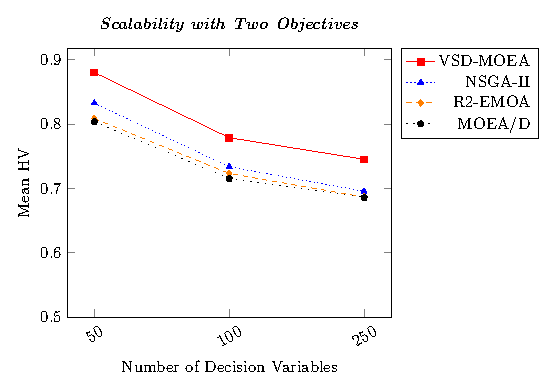
\includegraphics[scale=0.72]{Images/Graphic-Scalability-2obj_tikz-figure0.eps} & 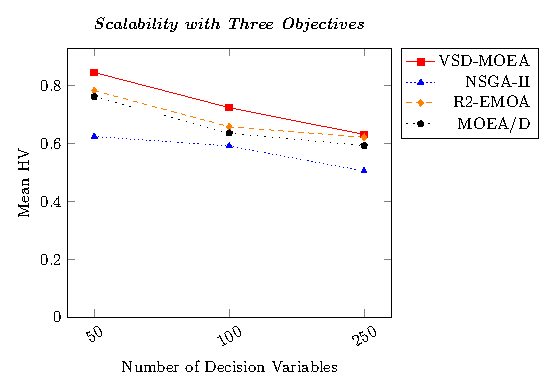
\includegraphics[scale=0.72]{Images/Graphic-Scalability-3obj_tikz-figure0.eps}
\end{tabular}
\caption{Mean of the \HV{} ratio for 35 runs for the two-objective (left side) and three-objective (right side) problems considering different numbers of variables}\label{fig:variable-decision-scalability}
\end{figure}

%\begin{figure}[t]
%\centering
%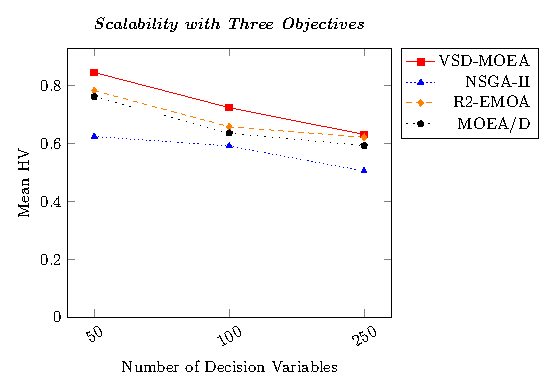
\includegraphics[scale=0.85]{Images/Graphic-Scalability-3obj_tikz-figure0.eps}
%\caption{Mean of the \HV{} ratio for 35 runs for the three-objective problems considering different numbers of variables} \label{fig:variable-decision-scalability-3obj}
%\end{figure}

In order to better understand this behavior, we selected problems WFG1 to WFG7.
%
The WFG test problems divide the variables into two kinds of parameters (this framework uses the term parameter instead of 
variable): the distance parameters and the position parameters.
%
Note that a parameter $i$ is a distance parameter when for all $\vec{\mathbf{x}}$, modifying $x_i$ results in a new solution 
that dominates $\vec{\mathbf{x}}$, is equivalent to $\vec{\mathbf{x}}$, or is dominated by $\vec{\mathbf{x}}$.
%
However, if $i$ is a position parameter, modifying $x_i$ in $\vec{\mathbf{x}}$ always results in a vector that is incomparable or 
equivalent to $\vec{\mathbf{x}}$~\citep{huband2005scalable}.
%
Additionally, note that we selected problems WFG1-WFG7 because their distance parameter values associated to all Pareto optimal solutions 
have exactly the same values:
%
\begin{equation}
   x_{i=k+1:n} = 2i \times 0.35
\end{equation}
%
This is very important because it has been shown that for these cases, state-of-the-art
\MOEAS{} might provoke a quick convergence in \textit{distance parameters}, resulting in an effect that is similar to 
premature convergence in the single-objective case~\citep{Joel:GDE3_CEC09,castillo2017multi}.

\begin{figure}[t]
\centering
\setlength{\tabcolsep}{0.0em}
\begin{tabular}{c c}
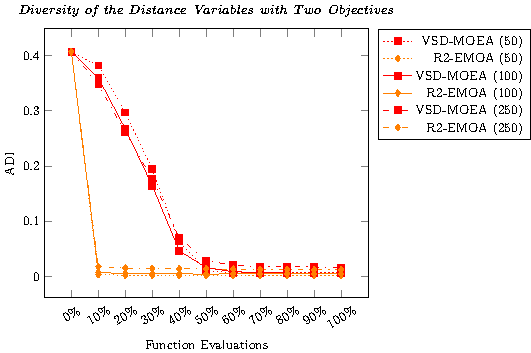
\includegraphics[scale=0.75]{Images/Graphic-Diversity_2obj_tikz-figure1.eps} & 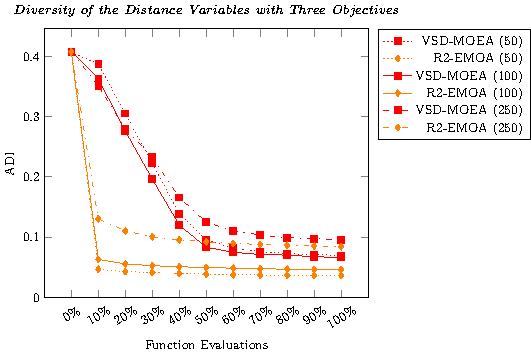
\includegraphics[scale=0.75]{Images/Graphic-Diversity_3obj_tikz-figure1.eps}
\end{tabular}
\caption{Evolution of ADI for problems WFG1-WFG7 with two and three objectives considering only the distance variables}\label{fig:Diversity}
\end{figure}

For each algorithm, we calculated the average (mean) Euclidean distance among individuals (ADI) in the population by considering only 
the distance parameters.
%
Figure~\ref{fig:Diversity} shows how the ADI evolves for the two-objective (left side) and three-objective (right side) problems.
%Figures~\ref{fig:Diversity_2obj} and~\ref{fig:Diversity_3obj} show how the ADI evolves for the two-objective and three-objective problems.
%
The behavior of \NSGAII{} and \MOEAD{} --- which are not included --- is similar to that of \RMOEA{} in terms of how the ADI evolves. 
%
Thus, to avoid saturating these figures, only the information for \VSDMOEA{} and \RMOEA{} with 50, 100 and 250 variables is shown.
%
The first obvious fact is that \VSDMOEA{} converges much slower than \RMOEA{}.
%
Accordingly, the difference between the diversity maintained in the first generation and that maintained after 10\% of the execution,
is much larger in \RMOEA{} than in \VSDMOEA{}.
%
In the case of \VSDMOEA{}, the decrease in ADI is quite linear until the halfway point of the execution.
%
This is due to the way in which the threshold distance value ($D_t$) is calculated.
%
Additionally, a closer inspection of the data reveals other important aspects that must be discussed. 
%
In the two-objective case, increasing the number of variables causes the diversity in the \RMOEA{} to increase slightly.
%
However, the amount of diversity is low even when using 250 variables, meaning that incorporating mechanisms to increase diversity --- as is done in \VSDMOEA{} ---
is very helpful.
%
In contrast, in the three-objective case, the amount of diversity in \RMOEA{} is not as low.
%
Moreover, increasing the number of variables yields a significant increase in the resulting ADI, meaning that in this case,
fast convergence is not an important issue.
%
These results show that, as the number of objectives and variables increases, \MOEAS{} tend to maintain a higher variable space diversity
in an implicit way, meaning that explicitly controlling the variable space diversity is probably not as important.
%

Finally, it is worth noting that we selected some problems to conduct long-term executions with 250 variables.
%
\VSDMOEA{} was able to further improve the results when using long-term executions, while the other state-of-the-art algorithms did not yield significant improvements.
%
This probably means that as technology evolves, allowing longer executions to be carried out in reasonable time frames,
the incorporation of explicit control of diversity will be even more important.
%
Note that this also happens in the single-objective case, where the benefits of explicitly controlling diversity appears only when using executions lasting
several weeks when dealing with large instances of the Traveling Salesman Problem~\citep{segura2015novel}.
%

%\begin{figure}[t]
%\centering
%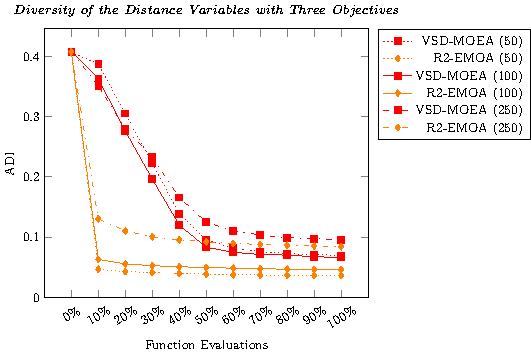
\includegraphics[scale=0.85]{Images/Graphic-Diversity_3obj_tikz-figure1.eps}
%\caption{Evolution of ADI for problems WFG1-WFG7 with three objectives considering only the distance variables}\label{fig:Diversity_3obj}
%\end{figure}

\subsection{Analysis of the Stopping criterion}

This section ilustrates the main reason behind the superiority of the \VSDMOEA{} against state-of-the-art algorithms in long-term executions.
%
As previously discussed, \EAS{} with explicit control of diversity often are more useful in long-term executions.
%
The fact that we selected a rather large stopping criterion in our first experiment might lead readers to think that \VSDMOEA{} is only
useful in extremely long-term executions;
%
however, this is not the case.
%
In this section we analyze the performance of \VSDMOEA{} and state-of-the-art algorithms with several stopping criteria, 
i.e., maximum number of function evaluations.
%
Three different ranges were explored for the stopping criterion.
%
Each range was split into ten equally distributed intervals, and experiments were run with each different number of function evaluations.
%
The ranges considered were $[2.5 \times 10^4, 2.5 \times 10^5]$, $[2.5 \times 10^5, 2.5 \times 10^6]$ and $[2.5 \times 10^6, 2.5 \times 10^7]$.
%
These ranges are referred to as short-term, middle-term and long-term executions, respectively.
%
Note that state-of-the-art algorithms can be executed just once (with $2.5 \times 10^7$ function evaluations) by saving the intermediate results.
%
However, \VSDMOEA{} makes decisions that depend on the stopping criteria, so independent executions were required for each stopping criterion.

\begin{figure}[t]
\centering
\setlength{\tabcolsep}{0.0em}
\begin{tabular}{cc}
\begin{tabular}{l}
 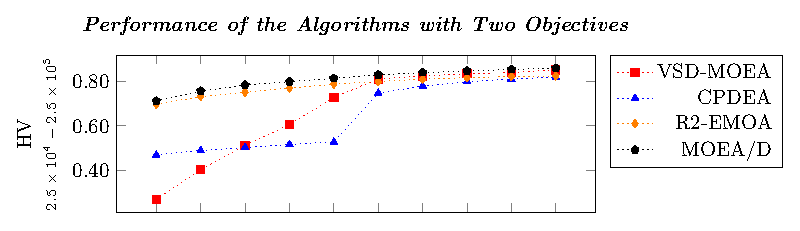
\includegraphics[scale=0.5]{Images/Time_tikz-figure0.eps}\\[0cm]%[-0.14cm] 
 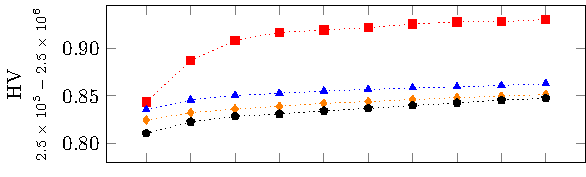
\includegraphics[scale=0.5]{Images/Time_tikz-figure1.eps}\\[0cm]%[-0.18cm]
 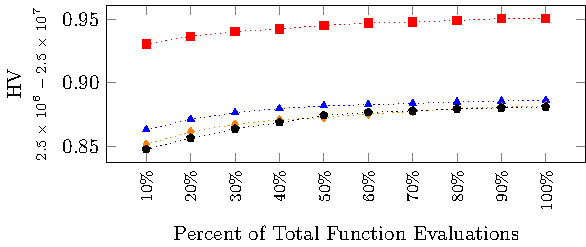
\includegraphics[scale=0.5]{Images/Time_tikz-figure2.eps}
\end{tabular}
& \begin{tabular}{l}
 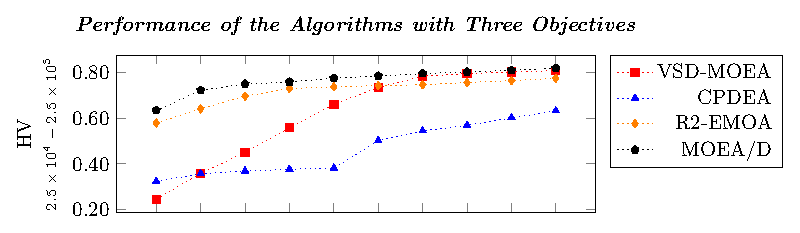
\includegraphics[scale=0.5]{Images/Time_tikz-figure3.eps}\\[0cm]%[-0.14cm] 
 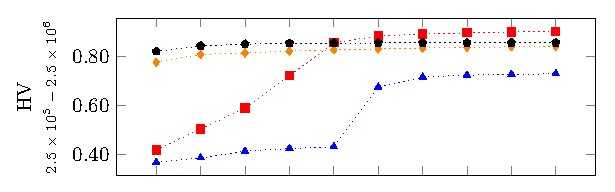
\includegraphics[scale=0.5]{Images/Time_tikz-figure4.eps}\\[0cm]%[-0.18cm]
 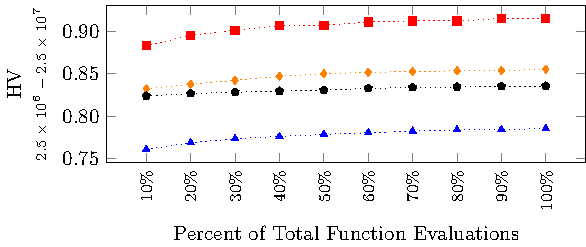
\includegraphics[scale=0.5]{Images/Time_tikz-figure5.eps}
\end{tabular}

\end{tabular}
\caption{Performance of \MOEAS{} for the problems with two objectives (left side) and three objectives (right side) considering three ranges for the stopping criterion: 
short-term (first row), middle-term (second row) and long-term (third row).}\label{fig:Performance_time}
\end{figure}

Figure~\ref{fig:Performance_time} shows the mean \HV{} ratio obtained with each \MOEA{} 
%Figures~\ref{fig:Performance_time_2obj} and~\ref{fig:Performance_time_3obj} show the mean \HV{} ratio obtained with each \MOEA{} 
with two and three objectives, respectively.
%
All the problems were considered to calculate this mean ratio.
%
Each figure is divided into three graphs corresponding to short-term, middle-term and long-term.
%
In the two-objective case, for the shortest executions, \VSDMOEA{} is not very competitive.
%
In the range $[2.5 \times 10^4, 7.5 \times 10^4]$, it exhibits the worst performance, meaning that for very short-term executions,
explicitly promoting additional diversity is not helpful.
%
When using $10^5$ function evaluations, the resulting \HV{} ratio is similar than that obtained by other methods.
%
Finally, when using more than $2.5 \times 10^5$ function evaluations, the \HV{} ratio obtained by \VSDMOEA{} is much higher than the one
obtained by other methods.
%
It is worth noting that \VSDMOEA{} is the only method that truly takes advantage of using long-term executions,
with the remaining methods just showing a slight improvement.
%
In the three-objective case, \VSDMOEA{} yields a lower \HV{} ratio than \RMOEA{} and \MOEAD{} in short-term executions,
but as more function evaluations are executed, the differences decrease.
%
In this case, after $5 \times 10^5$ function evaluations, the performance of \VSDMOEA{} is similar to that of \RMOEA{}.
%
Finally, as in the two-objective case, with additional function evaluations, the differences between \VSDMOEA{} and the remaining
algorithms increase in favor of \VSDMOEA{}.
%
Thus, while the most important benefits arise in long-term executions, users can benefit from \VSDMOEA{} even in shorter executions.


\subsection{Analysis of the Initial Threshold Value}

One of the disadvantages of including a strategy for controlling diversity is that this is usually done at the expense of
incorporating additional parameters in the \EA{} designed.
%
In the case of \VSDMOEA{}, the initial threshold value ($D_I$) must be set.
%
The higher this value is, the greater the exploration of the decision variable space.
%
Note that in all the previous experiments, $D_I = 0.4$ was used.
%
This value was selected based on some preliminary experiments.
%
This section is devoted to analyzing the performance of \VSDMOEA{} when using different $D_I$ values. 
%
Note that, since normalized distances are used, the maximum difference that can appear is $1$.
%
Additionally, note that when $D_I$ is set to 0, no individual is penalized on the basis of its decision
variable space diversity contribution,
so \VSDMOEA{} would behave like a more traditional \MOEA{}.
%
As a result, the values $D_I = \{0.0, 0.1, 0.2, 0.3, 0.4, 0.5, 0.6, 0.7, 0.8, 0.9\}$ were tested.
%
As in previous experiments, the whole set of benchmark problems was used and
the stopping criterion was set to $2.5 \times 10^7$ function evaluations.

\begin{figure}[t]
\centering
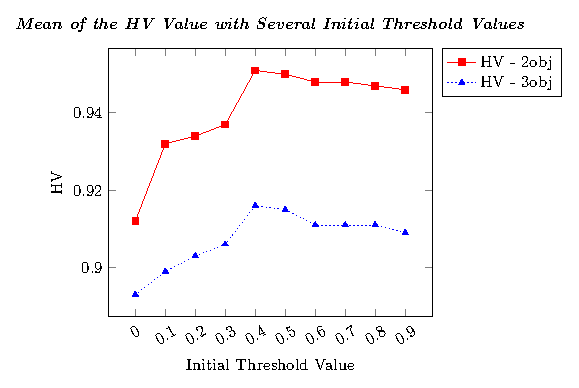
\includegraphics[scale=0.85]{Images/Graphic-Initial-Distance_tikz-figure0.eps} \\
\caption{Mean of \HV{} values taking into account all the problems with several initial threshold values}\label{fig:Initial-distance-factor}
\end{figure}

Figure~\ref{fig:Initial-distance-factor} shows the mean \HV{} ratio obtained for both the two-objective 
and the three-objective case.
%
Note that even when $D_I$ is set to $0$, \VSDMOEA{} yielded better \HV{} ratios than other 
state-of-the-art algorithms (see Tables~\ref{tab:StatisticsHV_2obj} and~\ref{tab:StatisticsHV_3obj}).
%
Specifically, the values were $0.912$ and $0.893$ for two and three objectives, respectively.
%
This means that the novel density estimator put forth in this paper is indeed helpful.
%
However, the increase in performance when using other $D_I$ values is clear.
%
The \HV{} ratio obtained quickly increases as higher $D_I$ values up to $0.4$ are used.
%
Then, with values in the range $[0.5, 0.9]$, the performance decreases slightly.
%
There is a large range of values where the performance is very good, meaning that 
the behavior of \VSDMOEA{} is quite robust.
%
Thus, properly setting this parameter is not a complex task.
%
%\begin{figure}[t]
%\centering
%\begin{tabular}{l}
% 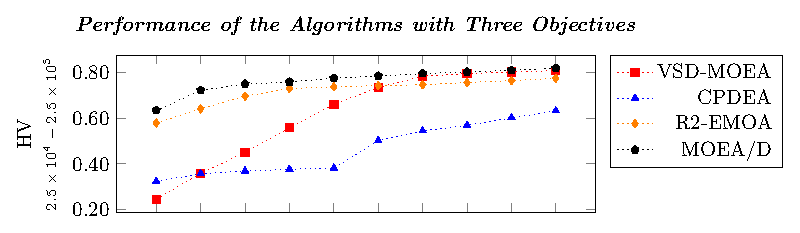
\includegraphics[scale=0.6]{Images/Time_tikz-figure3.eps}\\[0cm]%[-0.14cm] 
% 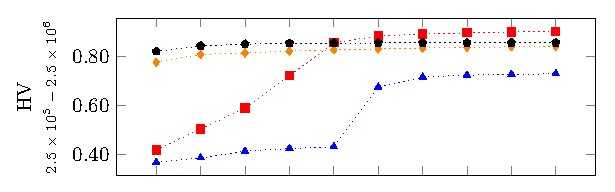
\includegraphics[scale=0.6]{Images/Time_tikz-figure4.eps}\\[0cm]%[-0.18cm]
% 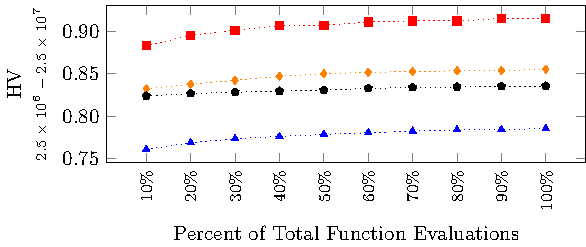
\includegraphics[scale=0.6]{Images/Time_tikz-figure5.eps}
%\end{tabular}
%\caption{Performance of \MOEAS{} for the problems with three objectives considering three ranges for the stopping 
%criterion: short-term (first row), middle-term (second row) and long-term (third row).}\label{fig:Performance_time_3obj}
%\end{figure}


